%% 
%% Copyright 2007-2020 Elsevier Ltd
%% 
%% This file is part of the 'Elsarticle Bundle'.
%% ---------------------------------------------
%% 
%% It may be distributed under the conditions of the LaTeX Project Public
%% License, either version 1.2 of this license or (at your option) any
%% later version.  The latest version of this license is in
%%    http://www.latex-project.org/lppl.txt
%% and version 1.2 or later is part of all distributions of LaTeX
%% version 1999/12/01 or later.
%% 
%% The list of all files belonging to the 'Elsarticle Bundle' is
%% given in the file `manifest.txt'.
%% 
%% Template article for Elsevier's document class `elsarticle'
%% with harvard style bibliographic references

%\documentclass[preprint,12pt,authoryear]{elsarticle}

%% Use the option review to obtain double line spacing
%% \documentclass[authoryear,preprint,review,12pt]{elsarticle}

%% Use the options 1p,twocolumn; 3p; 3p,twocolumn; 5p; or 5p,twocolumn
%% for a journal layout:
%% \documentclass[final,1p,times,authoryear]{elsarticle}
%% \documentclass[final,1p,times,twocolumn,authoryear]{elsarticle}
%% \documentclass[final,3p,times,authoryear]{elsarticle}
%% \documentclass[final,3p,times,twocolumn,authoryear]{elsarticle}
%% \documentclass[final,1p,times,authoryear]{elsarticle}


%%
%% Cleaned Elsevier manuscript
%%

\documentclass[final,1p,times]{elsarticle}

\usepackage{amsmath}
\usepackage{amssymb}
\usepackage{booktabs}
\usepackage{array}
\usepackage{float}
\usepackage[section]{placeins}
\usepackage[ruled]{algorithm2e}
\usepackage{graphicx}
\usepackage{tikz}
\usepackage[numbers,sort&compress]{natbib}
\usetikzlibrary{positioning,arrows.meta,shapes.multipart,fit,backgrounds,calc}

\DontPrintSemicolon
\SetAlgoNoEnd
\LinesNumberedHidden

\journal{Knowledge-Based Systems}

\begin{document}

\begin{frontmatter}

\title{Emotion-Aware Broadcast News Analytics: An Integrated Deep Learning Pipeline for Topic Extraction, Sentiment Intensity Scaling, and Semantic-Preserving Regulation}

\author[first]{Tayyab Rehman}
\ead{tayyab.rehman@graduate.univaq.it}

\affiliation[first]{organization={Department of Information Engineering, Computer Science, and Mathematics, University of L'Aquila},
addressline={Via Vetoio},
city={L'Aquila},
postcode={67100},
country={Italy}}

\author[Second]{Muzzamil Mustafa}
\ead{muzzamilmustafa0@gmail.com}

\affiliation[Second]{organization={Department of Information Engineering, Computer Science and Mathematics, Università degli Studi dell'Aquila},
addressline={Via Vetoio},
city={L'Aquila},
postcode={67100},
country={Italy}}

\begin{abstract}

The rapid growth of digital news broadcasting has increased public exposure to emotionally amplified media narratives. While sentiment analysis is widely used to evaluate emotional tone in news content, most existing approaches focus on polarity classification and overlook the measurement of emotional intensity, preventing the detection of exaggerated emotional framing in broadcast news. This paper proposes an Emotion-Aware News Analytics framework designed to detect, quantify, and regulate emotional amplification in broadcast news. The system processes multimedia news through a multi-stage pipeline: automatic speech recognition, semantic segmentation, topic modeling, contextual sentiment classification, and an iterative text-rewriting module that reduces excessive emotional intensity while preserving semantic content. The pipeline transforms raw broadcast videos into structured datasets containing topic labels, sentiment polarity, and sentiment intensity (operationalized via the confidence score of a transformer-based sentiment classifier). Segments exceeding a predefined threshold undergo semantic-preserving rewriting to attenuate emotional intensity. The framework combines a knowledge-driven component (topic taxonomy and amplification threshold) with data-driven models to support expert decision-making in media monitoring and content moderation. Experiments on 120 broadcast news videos (15 months) yielded 639 semantically segmented items. Results indicate that approximately 45.2\% of segments exhibited high-confidence emotional amplification; the rewriting mechanism reduced sentiment intensity by an average of $\Delta\sigma \approx 0.19$ (SD $= 0.08$, 95\% CI [0.17, 0.21]) while preserving semantic meaning. A pilot human evaluation (40 segments, two raters) reported 87.5\% semantic preservation and 82.5\% perceived intensity reduction ($\kappa \approx 0.72$ and 0.68). A conflict-centric case study (62 segments) confirmed topic-dependent amplification and that the system attenuates avoidable exaggeration while preserving factual severity. The primary contribution is the integration of existing NLP techniques into a reproducible, knowledge-aware end-to-end pipeline rather than a new learning algorithm. The framework supports rather than replaces human experts and provides a scalable approach for detecting and moderating emotionally amplified news narratives in digital media ecosystems.

\end{abstract}

\begin{keyword}
News Analytics \sep Sentiment Regulation \sep Topic Modeling \sep Zero-Shot Classification \sep Emotional Intensity Scaling \sep Knowledge-Based System \sep Decision Support \sep NLP Pipeline \sep Media Psychology
\end{keyword}

\end{frontmatter}

% ============================================================
\section{Introduction}
\label{introduction}

The rapid digital transformation of news dissemination has fundamentally reshaped how information is produced, distributed, and consumed \cite{newman2025digital}. Online platforms and broadcast multimedia channels have largely replaced traditional print journalism, providing real-time updates, global accessibility, and visually enriched storytelling \cite{lamai2025broadcast}. While this transition has enhanced informational reach and engagement, it has simultaneously intensified emotional exposure. Contemporary news reporting frequently incorporates vivid imagery, tonal emphasis, and emotionally charged framing, which can significantly influence cognitive processing and public perception \cite{rakhimboeva2025application}. From a psychological and communication-theoretic perspective, emotionally amplified information exerts stronger effects on attention, memory retention, and risk perception than neutrally framed content. Repeated exposure to highly polarized narratives such as crisis reporting, geopolitical conflict, economic instability, or disaster coverage may reinforce negativity bias and contribute to elevated stress levels \cite{harliantara2026media,burton2025anxiety,soroka2026negativity}. Conversely, excessively optimistic or sensationally positive narratives may inflate public expectations and generate psychological strain when anticipated outcomes fail to materialize \cite{stroud2010polarization}. These dynamics suggest that emotional amplification, irrespective of polarity direction, plays a critical role in shaping cognitive and affective responses \cite{xu2025emotion}.

In computational media analytics, sentiment analysis and topic modeling have become widely adopted tools for examining large-scale news corpora. Context-aware and AI-driven approaches integrating traditional and transformer-based models have been applied to threat detection and federated intrusion detection \cite{contextawarethreat2024,fflids2024}. Transformer-based architectures have substantially improved contextual sentiment detection, enabling fine-grained polarity classification across domains \cite{vaswani2017attention,devlin2019bert,liu2019roberta}. Similarly, probabilistic and neural topic modeling techniques allow structured exploration of thematic evolution \cite{dubey2025contextualized}. However, existing approaches predominantly focus on discrete sentiment polarity classification (positive, negative, neutral) and overlook the modeling of emotional intensity amplification. Consequently, current systems quantify emotional direction but fail to capture the magnitude of exaggeration or its potential psychological implications \cite{kumar2025cross}.

The growing reliance on short-form broadcast segments further contributes to this phenomenon. Modern headline news formats typically compress multiple complex events into brief segments lasting only a few seconds or minutes \cite{fahima2025sentiment}. This compression encourages linguistic intensification, where strong adjectives, urgent phrasing, and simplified narrative structures are used to quickly convey perceived importance. Consequently, viewers are often exposed to emotionally condensed narratives that may influence perception of risk, urgency, and social instability. Understanding how such framing patterns emerge and how they evolve over time requires computational tools capable of analyzing news content at a fine-grained segment level rather than treating entire broadcasts as homogeneous textual documents \cite{bednarek2025attitude}. From a methodological standpoint, the integration of natural language processing, machine learning, and multimedia analysis provides new opportunities for systematic investigation of emotional dynamics in news content. Advances in automatic speech recognition, transformer-based language models, and large-scale representation learning enable researchers to extract structured information from previously unstructured broadcast media streams. These developments allow the construction of computational pipelines that not only detect sentiment but also quantify patterns of emotional intensity across topics, time periods, and narrative contexts. Such approaches open new possibilities for large-scale monitoring of media tone and for the development of analytical tools that support responsible and psychologically aware media ecosystems \cite{castillo2025media}.

Furthermore, most prior research concentrates on textual news articles rather than broadcast news videos, which now represent a dominant format in digital media ecosystems. Video-based news introduces additional analytical challenges, including automatic speech recognition variability, segment-level thematic transitions, multimodal contextual dependencies, and temporally evolving emotional cues \cite{navarrete2025closer}. Document-level sentiment classification is therefore insufficient for understanding fine-grained emotional dynamics within broadcast news segments. Despite increasing societal concern regarding media-induced stress and anxiety and the need for governance of automated content systems \cite{waldman2022governing}, existing computational frameworks do not incorporate mechanisms to regulate exaggerated sentiment while preserving informational integrity. The absence of intensity-aware modeling and regulation mechanisms constitutes a critical gap in current multi-modal news analytics research \cite{wang2025cross}.

To address these limitations, this study proposes an Emotion-Aware Multi-modal News Analytics Framework designed to detect, quantify, and regulate emotional amplification in broadcast news content. The framework is conceived as a knowledge-based decision-support system: it combines a knowledge-driven component (a predefined topic taxonomy and an amplification threshold that encodes expert or policy constraints) with data-driven models (ASR, segmentation, topic inference, sentiment analysis, and semantic-preserving rewriting) to support editors, moderators, or analysts in identifying and optionally attenuating high-amplification segments. The proposed pipeline integrates automatic speech recognition for transcript generation, semantic segmentation for segment-level structuring, transformer-based contextual sentiment modeling, and topic extraction for thematic analysis. In contrast to conventional sentiment classifiers, the framework introduces an emotional amplification modeling component that estimates sentiment intensity beyond polarity. When emotional extremity exceeds an adaptive threshold, a semantic-preserving normalization mechanism is applied to reduce amplification while maintaining factual meaning; the system supports rather than replaces human judgment.

\begin{table}[H]
\centering
\caption{Key concepts and terminology introduced in the study}
\label{tab:intro_terms}
\scriptsize
\setlength{\tabcolsep}{3pt}
\renewcommand{\arraystretch}{1.1}
\begin{tabular}{p{2.3cm} p{1.6cm} p{3.6cm} p{3.0cm}}
\hline
\textbf{Term} & \textbf{Category} & \textbf{Description} & \textbf{Relevance to Study} \\
\hline
Digital News Ecosystem & Media System &
The modern information environment in which news is distributed through online platforms, streaming services, and multimedia broadcasting channels. &
Provides the context in which emotionally intensified news content is produced and consumed. \\

Broadcast News Video & Media Format &
A multimedia news format combining spoken narration, visuals, and text overlays to deliver short-form news reports. &
Serves as the primary data source analyzed in this research. \\

Emotional Amplification & Cognitive / Media &
The process by which news narratives emphasize emotional tone through linguistic framing, vocal emphasis, or visual storytelling. &
Central concept examined in the proposed framework. \\

Sentiment Polarity & NLP Concept &
The directional classification of sentiment into categories such as positive, negative, or neutral. &
Forms the baseline emotional signal used for further intensity analysis. \\

Sentiment Intensity & NLP Metric &
A quantitative representation of how strongly a sentiment is expressed in a given text segment. &
Used to measure emotional amplification beyond simple polarity classification. \\

Semantic Segmentation & Text Processing &
The decomposition of a continuous transcript into smaller semantically coherent units representing individual news items. &
Enables fine-grained analysis at the segment level rather than at the full document level. \\

Topic Modeling & Text Mining &
A probabilistic technique used to identify latent thematic structures within a collection of documents or text segments. &
Used to identify dominant news themes within broadcast segments. \\

Transformer-Based Sentiment Analysis & Deep Learning &
A contextual language modeling approach using transformer architectures to infer sentiment from text. &
Provides contextual sentiment predictions used to estimate emotional tone. \\

Automatic Speech Recognition (ASR) & Speech Processing &
A computational technique that converts spoken audio into textual transcripts. &
Enables analysis of spoken broadcast news content. \\

Sentiment Attenuation & Text Generation &
A controlled rewriting procedure that reduces emotional intensity while preserving semantic meaning. &
Used to moderate emotionally amplified news segments. \\

Computational Media Analytics & Research Field &
An interdisciplinary field combining natural language processing, machine learning, and media studies to analyze digital news data. &
Provides the broader research context of the proposed framework. \\
\hline
\end{tabular}
\end{table}

\subsection{Research Motivation}

The motivation for this work arises from three converging developments. First, the exponential growth of multimedia news broadcasting has created large-scale unstructured data requiring automated and scalable analysis. Second, advances in transformer-based language models and multi-modal representation learning now enable contextual sentiment modeling at fine granularity. Third, growing empirical evidence linking emotionally amplified news exposure to psychological stress highlights the need for emotion-aware computational media systems. These factors collectively underscore the necessity of extending sentiment analysis beyond polarity detection toward emotional intensity modeling and regulation.

\subsection{Objectives}

The overarching objective of this research is to develop an emotion-aware computational framework capable of analyzing broadcast news at fine-grained temporal resolution while mitigating emotionally exaggerated language. Specifically, the study aims to:
\begin{enumerate}
    \item Construct an automated pipeline for ingesting and transcribing broadcast news videos.
    \item Perform segment-level semantic structuring to enable granular analysis.
    \item Extract and track topic distributions over time for longitudinal media analysis.
    \item Model contextual sentiment with explicit emotional intensity estimation.
    \item Regulate exaggerated sentiment through semantic-preserving normalization.
    \item Generate structured temporal datasets supporting reproducible evaluation and trend analysis.
\end{enumerate}

\subsection{Contributions}

The main contributions of this paper are summarized as follows:
\begin{enumerate}
    \item We formalize the problem of emotional amplification modeling in broadcast news analytics and propose a quantitative intensity estimation mechanism (operationalized via classifier confidence) extending conventional polarity-based sentiment frameworks.
    \item We develop a segment-level multi-modal news analysis pipeline integrating speech transcription, semantic segmentation, contextual transformer-based sentiment modeling, and topic extraction.
    \item We design a semantic-preserving sentiment regulation strategy that reduces exaggerated emotional intensity while maintaining factual and contextual integrity.
    \item We construct structured temporal topic--sentiment representations enabling longitudinal media narrative analysis and emotional trend tracking.
    \item We provide empirical validation demonstrating the effectiveness of the proposed framework in detecting and mitigating emotional polarization in broadcast news content.
\end{enumerate}

% ============================================================
\section{Related Work}

Recent advances in computational media analysis have shifted the focus from static sentiment classification toward a deeper understanding of narrative framing, emotional amplification, and multi-modal information dynamics. Contemporary research increasingly combines contextual language models, topic evolution techniques, and cross-modal learning frameworks to capture how emotional signals propagate within modern news ecosystems. The most recent literature (2023–2026) can be broadly categorized into four research directions: contextual sentiment modeling, multi-modal news analysis, neural topic evolution, and bias detection with mitigation strategies.

\subsection{Contextual Sentiment and Emotional Intensity}

Recent studies have emphasized that sentiment polarity alone is insufficient for accurately representing emotional framing in journalistic discourse. A comprehensive benchmarking study of sentiment analysis models applied to multilingual news corpora \cite{zanoli2025benchmarking} shows that large language models outperform classical machine learning approaches such as SVM and CNN architectures; however, they remain susceptible to neutrality bias, where objectively reported tragic events are misinterpreted as negative opinion. Similarly, \cite{areia2025sentiment} introduced a seven-level sentiment intensity scale designed to capture the varying degrees of emotional gravity present in research and media attention, demonstrating that sentiment intensity provides stronger predictive power for real-world impact than simple polarity-based classification. Complementary evidence is provided by \cite{kim2025news}, who analyzed emotional dynamics in financial news and social media. Their findings reveal that traditional news media often acts as an emotional stabilizing mechanism, while social media platforms exhibit significantly higher sentiment volatility. Collectively, these studies demonstrate the increasing importance of contextual sentiment modeling and intensity-aware analysis. Nevertheless, most existing approaches remain focused on detection rather than computational mechanisms for regulating exaggerated emotional framing.

\subsection{Multi-modal Framing and Video Analytics}

The rapid growth of video-based news consumption has accelerated research into multi-modal sentiment analysis frameworks that integrate textual, visual, and acoustic information. \cite{arora2025multi} introduced a multi-modal framing analysis framework capable of identifying discrepancies between textual narratives and accompanying visual imagery, revealing visual–textual dissonance where emotionally charged images amplify the perceived severity of otherwise neutral textual statements. \cite{malik2025multimodal} proposed a cross-modal affect recognition model combining wav2vec2 for audio processing and ViViT for visual analysis, demonstrating that non-verbal signals such as vocal pitch variation and facial tension contribute significantly to the emotional perception of broadcast news segments. Further insights into short-form video dissemination were provided by \cite{he2025multimodal}, who developed a multimodal sentiment framework for social video platforms. The study found that emotional engagement in short-form news videos is strongly influenced by audience interaction signals and visual saturation rather than the factual density of spoken transcripts. A broader overview of audio–visual fusion methods in video sentiment analysis was presented by \cite{baberwal2025systematic}, who systematically reviewed multi-modal sentiment modeling strategies and highlighted the lack of domain-specific datasets for broadcast news analytics. Reliable transcription remains a foundational component of broadcast analysis pipelines. \cite{radford2025whisper} introduced Whisper, a large-scale automatic speech recognition system trained using weak supervision. Whisper demonstrates near-human transcription performance across diverse acoustic conditions and has become widely adopted in multimedia analytics pipelines. Despite these advancements, existing multi-modal approaches primarily focus on emotion classification rather than modeling emotional intensity or regulating amplification in broadcast narratives.

\subsection{Neural Topic Modeling and Temporal Evolution}

Topic modeling techniques play a central role in identifying emerging narratives and tracking thematic evolution in large news datasets. \cite{boutaleb2024bertrend} introduced an online topic discovery framework (BERTrend) capable of detecting emerging signals within streaming textual data using density-based clustering techniques such as HDBSCAN. \cite{schweizer2025political} applied neural topic modeling techniques to analyze sentiment patterns in state-backed media outlets. Their results revealed strong coupling between geopolitical topics and sentiment framing, suggesting that narrative tone may be strategically aligned with political messaging. Recent methodological developments have also explored guided topic discovery approaches. Emerging reports in data science literature emphasize the growing use of seeded topic modeling techniques, where large language models assist in filtering noisy topics and improving semantic coherence in real-time analysis pipelines. These developments demonstrate the importance of combining topic modeling with contextual semantic representations in order to capture evolving narrative structures in modern news media.

\subsection{Bias Detection and Mitigation}

Recent research has also focused on detecting and mitigating bias introduced by automated systems in journalistic workflows. \cite{germani2025source} demonstrated that large language models evaluate identical news content differently depending on the attributed source of the text, with attribution to artificial intelligence significantly reducing perceived credibility scores. \cite{startari2025ethos} proposed identity-blind evaluation protocols designed to minimize such biases when assessing news content generated or edited by automated systems. Policy-level research has also highlighted the growing societal risks associated with generative media technologies. \cite{newman2025digital} reported that public trust in AI-generated journalism remains limited, particularly when AI systems assume the role of visible presenters or anchors. Complementary policy analyses from European institutions warn that generative artificial intelligence significantly lowers the cost of producing emotionally persuasive disinformation campaigns. These findings underscore the importance of computational systems capable not only of detecting bias but also of moderating emotionally amplified narratives.

Together, these studies illustrate that the current frontier of computational media research lies in the integration of bias detection, emotional intensity modeling, and automated content regulation mechanisms.

\begin{table}[H]
\centering
\caption{Summary of related work: techniques, key contributions, datasets, and limitations compared to the proposed framework.}
\label{tab:related_work}
\scriptsize
\setlength{\tabcolsep}{4pt}
\renewcommand{\arraystretch}{1.15}
\begin{tabular}{c p{2.1cm} p{3.4cm} p{2.4cm} p{3.2cm}}
\toprule
\textbf{Ref.} & \textbf{Technique} & \textbf{Key contributions} & \textbf{Dataset} & \textbf{Limitation} \\
\midrule
\cite{zanoli2025benchmarking} & Benchmarking ML for sentiment & Comparison of LLMs vs.\ SVM/CNN on sentiment; neutrality bias in news & Multilingual news articles & Detection only; no intensity regulation \\
\cite{areia2025sentiment} & Sentiment intensity scale & Seven-level intensity for research attention; stronger predictive power than polarity & Altmetric / research attention & No regulation mechanism \\
\cite{kim2025news} & News vs.\ social media sentiment & Emotional dynamics in financial news; traditional media as stabilizer & Big tech stock, news \& social media & Polarity focus; no attenuation \\
\cite{arora2025multi} & Multi-modal framing analysis & Visual–textual dissonance; image–text discrepancy in news & News with imagery & Emotion classification only \\
\cite{malik2025multimodal} & Multimodal emotion detection & wav2vec2 + ViViT; non-verbal cues for affect & Audio–visual data & No semantic-preserving regulation \\
\cite{he2025multimodal} & Multimodal sentiment (short video) & Audience interaction \& visual saturation vs.\ factual density & Short-form social video & No broadcast news; no attenuation \\
\cite{radford2025whisper} & ASR (Whisper) & Large-scale weak supervision; near-human transcription & Diverse audio & Transcription only; no downstream regulation \\
\cite{boutaleb2024bertrend} & Online topic discovery (BERTrend) & HDBSCAN; emerging signals in streaming text & Streaming textual data & Topics only; no sentiment intensity \\
\cite{schweizer2025political} & Neural topic + sentiment & Geopolitical topics \& sentiment coupling in state media & State-backed media & No intensity modeling or regulation \\
\cite{germani2025source} & Source framing \& LLM bias & Attribution changes perceived credibility of identical content & LLM evaluation data & Bias detection; no content regulation \\
\cite{startari2025ethos} & Identity-blind evaluation & Protocols to reduce bias when assessing AI-generated news & News evaluation & No rewriting or attenuation \\
\cite{newman2025digital} & Trust in AI journalism & Public trust limits for AI presenters/anchors & Survey / policy report & Policy focus; no technical regulation \\
\midrule
\textbf{Ours} & \textbf{EAR framework} & \textbf{ASR + semantic segmentation + LDA–embedding topics + transformer sentiment + confidence-based intensity + semantic-preserving attenuation} & \textbf{120 broadcast videos; 639 segments (YouTube, 15 months)} & \textbf{Single source; English only; threshold $\theta$ and $G(\cdot)$ are design choices} \\
\bottomrule
\end{tabular}
\end{table}

\subsection{Research Gap}

Despite extensive work in sentiment analysis, multi-modal modeling, topic extraction, and emotional dynamics, three key limitations remain: (i) most approaches focus on polarity classification rather than emotional intensity modeling, (ii) broadcast news video analysis remains underexplored compared to textual news, and (iii) no prior research integrates sentiment intensity estimation with semantic-preserving regulation. These gaps motivate the development of the proposed Emotion-Aware Multi-modal News Analytics Framework.

% ============================================================
\section{Methodology}
\label{sec:methodology}

This study proposes a multi-stage computational framework for analyzing daily headline news videos with the aim of jointly modeling thematic content and emotionally amplified language at the segment level. The central objective of the framework is to transform unstructured broadcast media into a structured analytical representation that captures the dominant topic of each news item, its sentiment polarity, and the intensity with which that sentiment is expressed over time. To achieve this, the proposed pipeline sequentially performs video acquisition, speech transcription, semantic segmentation, linguistic preprocessing, topic inference, sentiment estimation, emotional amplification detection, semantic-preserving attenuation, and structured temporal storage. The complete operational workflow is summarized in Algorithm~\ref{alg:pipeline}, while the overall system architecture is illustrated in Fig.~\ref{fig:mechanism}. Formally, the input to the framework is a collection of news videos
\begin{equation}
\mathcal{V} = \{v_1, v_2, \dots, v_N\},
\end{equation}
where each video is associated with a publication date and subsequently mapped into a set of structured segment-level analytical records.

\subsection{Research Design and Data Acquisition}

The study follows a quantitative observational design in which broadcast news content is collected and analyzed without any manipulation of the original media. This design is appropriate because the goal is to model naturally occurring editorial framing rather than artificially generated discourse. Let $\mathcal{V}=\{v_1,v_2,\dots,v_N\}$ denote the set of collected headline videos over the observation period, where $N$ is the total number of retrieved broadcasts, and let $d_i$ represent the publication timestamp associated with video $v_i$. Each video is obtained programmatically through the YouTube Data API using a deterministic retrieval strategy that ensures reproducibility, consistency of selection criteria, and acquisition of the highest available stream quality. In this formulation, every video $v_i$ is treated as an authentic observation of real-world broadcast media output, and the ordered pair $(v_i,d_i)$ constitutes the primary temporal input to the downstream analytical pipeline. The data acquisition stage therefore establishes the foundational mapping from raw online video streams to a temporally indexed corpus suitable for computational media analysis.

\subsection{Speech-to-Text Transcription and Semantic Segmentation}

Since the source material is multimedia news content, the first transformation stage converts speech into text using an automatic speech recognition model. For each collected video $v_i$, the corresponding transcript is generated as
\begin{equation}
T_i = \mathrm{ASR}(v_i),
\end{equation}
where $T_i$ denotes the textual sequence obtained from the spoken audio of the video. However, daily headline broadcasts typically consist of multiple short stories presented within a single program, and therefore treating $T_i$ as a single analytical document would introduce topic leakage and sentiment contamination across unrelated narratives. To preserve story boundaries and improve interpretability, each transcript is partitioned into semantically coherent discourse segments,
\begin{equation}
T_i \rightarrow \mathcal{S}_i = \{s_{i1}, s_{i2}, \dots, s_{im_i}\},
\end{equation}
where $m_i$ denotes the number of identified segments in video $v_i$, and each segment $s_{ij}$ corresponds to a distinct news item. Segment boundaries are detected by a three-step procedure: (i) \emph{sentence-level splitting} of the ASR output into sentences; (ii) \emph{transition detection} using cue phrases (e.g., anchor lead-ins, topic-shift markers) and, when available, silence or pause boundaries from the ASR timestamps; (iii) \emph{optional merging} of adjacent sentence blocks whose embedding-based semantic similarity exceeds a threshold, so that each final segment forms a coherent narrative unit. This discourse-aware partitioning yields segments that align with editorial story boundaries in headline news. The result is a segment-level representation that aligns more closely with the editorial structure of headline news and forms the basis for all subsequent topic and sentiment inference steps described in Algorithm~\ref{alg:pipeline}.

\subsection{Text Normalization and Linguistic Preprocessing}

Before applying statistical and neural language models, each segment is normalized to reduce lexical sparsity and improve modeling stability. Let $\tilde{s}_{ij}$ denote the preprocessed form of segment $s_{ij}$, obtained by applying a preprocessing function that includes tokenization, stop-word removal, and lemmatization. This transformation is expressed as
\begin{equation}
\tilde{s}_{ij} = f_{\mathrm{prep}}(s_{ij}).
\end{equation}
The purpose of this stage is not to alter the semantic meaning of the segment, but rather to reduce morphological variation and remove linguistically redundant elements that may negatively affect probabilistic topic modeling and similarity-based semantic refinement. By converting inflected forms into their normalized lexical representations, the framework improves consistency across segments and supports more reliable estimation of latent thematic structure. As reflected in Algorithm~\ref{alg:pipeline}, the normalized segment $\tilde{s}_{ij}$ is the immediate input to the topic assignment procedure described in Algorithm~\ref{alg:topicassign}.

\subsection{Topic Inference via Probabilistic Modeling with Semantic Refinement}

Topic inference is performed through a hybrid procedure that combines probabilistic topic modeling with semantic refinement based on pretrained embeddings. LDA is trained once on the full corpus of all preprocessed segments (from all videos) to learn $K$ latent topics; then, for each segment $\tilde{s}_{ij}$, we infer the posterior topic distribution $P(z_k \mid \tilde{s}_{ij})$ and obtain the dominant topic. Under the LDA generative assumption, the probability of a word $w$ in a segment $\tilde{s}_{ij}$ is given by
\begin{equation}
P(w \mid \tilde{s}_{ij}) = \sum_{k=1}^{K} P(w \mid z_k)\,P(z_k \mid \tilde{s}_{ij}),
\end{equation}
where $z_k$ denotes the $k$-th latent topic. The dominant latent topic is obtained through maximum posterior assignment,
\begin{equation}
\tau_{ij}^{\mathrm{LDA}} = \arg\max_k P(z_k \mid \tilde{s}_{ij}).
\end{equation}
Representative words $\mathcal{W}_{ij}$ for this topic are taken as the top-$q$ words by $P(w \mid z_{\tau_{ij}^{\mathrm{LDA}}})$, where $q$ is a fixed parameter (e.g., $q=10$) set in the experimental configuration. Although this representation captures thematic structure, the resulting latent topics are often not directly interpretable in a news analytics setting. To address this limitation, a semantic refinement step is introduced using pretrained word embeddings. Let $\mathbf{v}_a$ and $\mathbf{v}_b$ denote embedding vectors corresponding to lexical items or topic descriptors $a$ and $b$. Their semantic proximity is computed using cosine similarity,
\begin{equation}
\mathrm{sim}(a,b)=\frac{\mathbf{v}_a \cdot \mathbf{v}_b}{\|\mathbf{v}_a\|\,\|\mathbf{v}_b\|}.
\end{equation}
Given a predefined topic taxonomy $\mathcal{C}$, the final topic label is selected by maximizing the average similarity between representative topic words $\mathcal{W}_{ij}$ and each category descriptor,
\begin{equation}
\tau_{ij}=\arg\max_{c \in \mathcal{C}} \frac{1}{|\mathcal{W}_{ij}|}\sum_{w \in \mathcal{W}_{ij}} \mathrm{sim}(w,c).
\end{equation}
This hybrid procedure, formally summarized in Algorithm~\ref{alg:topicassign}, improves interpretability, stabilizes topic assignment under vocabulary variation, and enables the mapping of probabilistic latent topics to a predefined set of domain-relevant news categories. The taxonomy $\mathcal{C}$ used in this study comprises the fifteen categories listed in Table~\ref{tab:taxonomy}. The number of LDA topics $K$ is set to match or exceed the taxonomy size. Embeddings for the cosine similarity $\mathrm{sim}(\cdot,\cdot)$ are obtained from a pretrained sentence encoder (in our experiments, \texttt{all-MiniLM-L6-v2} from the sentence-transformers library) so that words and category descriptors share a consistent semantic space.

\begin{table}[H]
\centering
\caption{Predefined topic taxonomy $\mathcal{C}$ used for segment-level classification}
\label{tab:taxonomy}
\small
\begin{tabular}{lll}
\hline
\textbf{Category} & \textbf{Category} & \textbf{Category} \\
\hline
International Affairs & Business & War \\
Politics & Economy & Health \\
Science & Technology & Environment \\
Education & Crime and Law & Culture and Society \\
Sports & Entertainment & Disaster and Crisis \\
\hline
\end{tabular}
\end{table}

\subsection{Sentiment Estimation and Emotional Amplification Scoring}

Sentiment inference is modeled as a three-class classification task over the label space
\begin{equation}
\mathcal{Y} = \{\mathrm{negative}, \mathrm{neutral}, \mathrm{positive}\}.
\end{equation}
For each segment $s_{ij}$, a pretrained transformer classifier produces posterior probabilities $P(y \mid s_{ij})$ for all sentiment classes. The predicted sentiment label is defined by the maximum posterior class,
\begin{equation}
y_{ij} = \arg\max_{y \in \mathcal{Y}} P(y \mid s_{ij}),
\end{equation}
while the corresponding dominant confidence score is
\begin{equation}
\sigma^{(0)}_{ij} = \max_{y \in \mathcal{Y}} P(y \mid s_{ij}).
\end{equation}
In conventional sentiment analysis, this confidence score is usually treated only as a measure of classifier certainty. In the present framework, however, $\sigma^{(0)}_{ij}$ is explicitly reinterpreted as a proxy for emotional amplification intensity. This distinction is essential because two segments can share the same sentiment polarity while differing substantially in the strength with which that polarity is expressed. Hence, the framework extends polarity analysis by treating confidence magnitude as an analytically meaningful indicator of affective extremity. We emphasize that $\sigma^{(0)}_{ij}$ is a \emph{computational proxy}: high confidence indicates that the classifier assigns strong polarity to the segment, which we interpret as correlated with the strength of emotional framing in the text. Classifier confidence may also reflect clear lexical sentiment signals, training-data bias, or model calibration rather than perceived emotional intensity; for example, a factual statement with strongly polarized wording or a segment with mild emotional tone could receive high confidence. We do not equate this score with human-rated emotional intensity. Validation against human judgments (Section~\ref{sec:experiments}) provides preliminary evidence of correlation; a more rigorous definition or empirical validation linking confidence to perceived amplification would strengthen the approach. This sentiment estimation stage is integrated into Algorithm~\ref{alg:pipeline} and provides the quantitative basis for deciding whether a segment requires attenuation.

\subsection{Sentiment Attenuation via Constrained Rephrasing}

A core contribution of the proposed framework is the introduction of an attenuation mechanism for emotionally amplified segments. Let $\theta$ denote a predefined amplification threshold such that a segment is classified as emotionally amplified whenever
\begin{equation}
\sigma^{(0)}_{ij} \ge \theta.
\end{equation}
For such segments, a generative rewriting function $G(\cdot)$ is used to produce a series of semantically equivalent but emotionally moderated reformulations. At iteration $r$, the rewritten candidate is represented as
\begin{equation}
s^{(r)}_{ij} = G(s_{ij}),
\end{equation}
and the corresponding sentiment confidence is recomputed as
\begin{equation}
\sigma^{(r)}_{ij} = \max_{y \in \mathcal{Y}} P(y \mid s^{(r)}_{ij}).
\end{equation}
The rewriting process is repeated up to a maximum of $R$ iterations, and the final regulated version is selected by minimizing the sentiment confidence over all generated candidates,
\begin{equation}
\sigma^{(*)}_{ij} = \min_{r \in \{1,\dots,R\}} \sigma^{(r)}_{ij}.
\end{equation}
This formulation casts attenuation as a constrained optimization process in which the objective is not to erase sentiment, but to reduce unnecessary affective amplification while preserving factual and semantic integrity. The current formulation does not impose explicit formal constraints (e.g., a minimum semantic similarity threshold or textual entailment between original and rewritten text); preservation of meaning is delegated to the prompt and the choice of $G(\cdot)$. Incorporating such constraints (e.g., BERTScore or entailment-based filters) to guarantee semantic equivalence is left for future work. The computational logic of this stage is described explicitly in Algorithm~\ref{alg:attenuate}, which shows how the framework iteratively rephrases text, scores each candidate, and retains the least amplified formulation.

\textbf{Implementation of $G(\cdot)$.} The rewriting function $G(\cdot)$ is implemented using a single pretrained paraphrase or instruction-tuned decoder fixed for all experiments; in our implementation we use \texttt{t5-base} (or an equivalent T5/BART paraphrase model) with a fixed prompt that asks the model to rephrase the segment while preserving facts and reducing emotionally charged wording. For each amplified segment $s_{ij}$, the model is prompted to produce a reformulation that (i) preserves the factual content and key entities of the original segment, (ii) reduces emotionally charged or intensifying wording (e.g., strong adjectives, hyperbolic phrases), and (iii) remains within a similar length to avoid truncation or padding artifacts. No manual editing is applied; each candidate $s^{(r)}_{ij}$ is generated in a single forward pass. The sentiment classifier is applied to the rewritten text only (without access to the original segment), so that $\sigma^{(r)}_{ij}$ reflects the perceived intensity of the candidate alone and avoids context bias. This design ensures that attenuation is fully automated and auditable.

\subsection{Structured Storage and Temporal Analysis}

After topic assignment, sentiment estimation, and optional attenuation, the framework constructs a structured dataset suitable for temporal and thematic media analytics. For each processed segment, the stored record includes its publication date, regulated text, assigned topic, sentiment label, initial confidence, and post-regulation confidence. Formally, the final dataset is written as
\begin{equation}
\mathcal{D} = \bigcup_{i=1}^{N} \{(d_i, s^{(*)}_{ij}, \tau_{ij}, y_{ij}, \sigma^{(0)}_{ij}, \sigma^{(*)}_{ij})\}_{j=1}^{m_i}.
\end{equation}
This structured representation enables temporal aggregation over publication dates and topics, allowing the analysis of how thematic prevalence and emotional intensity evolve over time. By computing grouped counts and score distributions across $(d_i,\tau_{ij})$ pairs, the framework supports downstream visualization of topic trends, sentiment shifts, and event-driven amplification patterns. In this sense, the structured dataset $\mathcal{D}$ serves not only as the final output of Algorithm~\ref{alg:pipeline}, but also as the primary analytical object for the experimental and temporal analyses reported later in the paper.

\subsection{Algorithmic Specification}

For reproducibility and computational transparency, the methodological pipeline is summarized through three compact algorithms. Algorithm~\ref{alg:pipeline} specifies the end-to-end transformation from daily broadcast videos to the structured dataset $\mathcal{D}$. Algorithm~\ref{alg:topicassign} details the hybrid topic assignment stage, in which latent probabilistic topics are mapped to an interpretable taxonomy using embedding-based semantic refinement. Algorithm~\ref{alg:attenuate} formalizes the sentiment attenuation mechanism that iteratively rephrases emotionally amplified segments and selects the candidate with minimum confidence. Together, these procedures define the computational backbone of the proposed emotion-aware news analytics framework.

\textbf{Knowledge representation and expert policy.} The framework embeds a knowledge-driven layer that governs interpretability and expert alignment. (i) The \emph{topic taxonomy} $\mathcal{C}$ (Table~\ref{tab:taxonomy}) encodes domain knowledge over news categories and ensures that topic labels are meaningful to end users. (ii) The \emph{amplification threshold} $\theta$ encodes expert or policy-defined tolerance for emotional intensity; segments above $\theta$ are flagged for attenuation. (iii) The \emph{semantic-preservation} constraint for the rewriting function $G(\cdot)$ and the \emph{maximum iterations} $R$ act as policy parameters that bound how much regulation is applied. These elements form the knowledge base of the system and can be adjusted by domain experts or institutional policy without retraining the underlying models.

\begin{table}[H]
\centering
\caption{Notation used in the proposed news analysis framework}
\label{tab:notation}
\small
\setlength{\tabcolsep}{3pt}
\renewcommand{\arraystretch}{1.08}
\begin{tabular}{p{3.7cm} p{5.9cm}}
\hline
\textbf{Symbol} & \textbf{Description} \\
\hline
$\mathcal{V}=\{v_i\}_{i=1}^{N}$ & Set of collected headline videos \\
$N$ & Total number of videos \\
$d_i$ & Publication date of video $v_i$ \\
$T_i$ & Transcript obtained via ASR \\
$\mathcal{S}_i=\{s_{ij}\}_{j=1}^{m_i}$ & Segmented transcript of $v_i$ \\
$m_i$ & Number of segments in broadcast $v_i$ \\
$s_{ij}$ & $j$-th news segment of video $v_i$ \\
$\tilde{s}_{ij}$ & Preprocessed segment text \\
$\mathcal{C}$ & Predefined topic taxonomy \\
$\tau_{ij}$ & Assigned topic label \\
$\mathcal{Y}$ & Sentiment label space \\
$y_{ij}$ & Predicted sentiment label \\
$\sigma^{(0)}_{ij}$ & Initial sentiment confidence score \\
$\sigma^{(*)}_{ij}$ & Post-regulation sentiment confidence \\
$\theta$ & Emotional amplification threshold \\
$R$ & Maximum rephrasing attempts \\
$G(\cdot)$ & Generative rephrasing function \\
$\mathcal{D}$ & Structured output dataset \\
\hline
\end{tabular}
\end{table}

\begin{algorithm}[H]
\caption{End-to-end daily news analysis and dataset construction}
\label{alg:pipeline}
\KwIn{Daily broadcasts $\mathcal{V}=\{v_1,\dots,v_N\}$ with dates $\{d_1,\dots,d_N\}$; taxonomy $\mathcal{C}$; threshold $\theta$; max attempts $R$.}
\KwOut{Structured dataset $\mathcal{D}$.}
$\mathcal{D}\leftarrow \emptyset$\;
\ForEach{$(v_i,d_i)$}{
    $T_i \leftarrow \mathrm{ASR}(v_i)$\;
    $\mathcal{S}_i \leftarrow \mathrm{Segment}(T_i)$\;
    \ForEach{$s_{ij}\in\mathcal{S}_i$}{
        $\tilde{s}_{ij}\leftarrow f_{\mathrm{prep}}(s_{ij})$\;
        $\tau_{ij}\leftarrow \mathrm{TopicAssign}(\tilde{s}_{ij},\mathcal{C})$\;
        $(y_{ij},\sigma^{(0)}_{ij})\leftarrow \mathrm{SentimentScore}(s_{ij})$\;
        $(s^{(*)}_{ij},\sigma^{(*)}_{ij})\leftarrow \mathrm{Attenuate}(s_{ij},\sigma^{(0)}_{ij},\theta,R)$\;
        $\mathcal{D}\leftarrow \mathcal{D}\cup\{(d_i,s^{(*)}_{ij},\tau_{ij},y_{ij},\sigma^{(0)}_{ij},\sigma^{(*)}_{ij})\}$\;
    }
}
\Return $\mathcal{D}$\;
\end{algorithm}

\begin{algorithm}[H]
\caption{TopicAssign: LDA topic inference with embedding-based taxonomy refinement}
\label{alg:topicassign}
\KwIn{Preprocessed segment $\tilde{s}$; taxonomy $\mathcal{C}$; LDA model trained on full corpus; embedding function $E(\cdot)$; number of topic words $q$ (e.g., $q=10$).}
\KwOut{Topic label $\tau \in \mathcal{C}$.}
Infer $P(z_k \mid \tilde{s})$ for $k=1,\dots,K$ using the trained LDA model; $z^* \leftarrow \arg\max_k P(z_k \mid \tilde{s})$\;
Obtain representative topic words $\mathcal{W}=\{w_1,\dots,w_q\}$ as the top-$q$ words by $P(w \mid z^*)$\;
\ForEach{$c\in\mathcal{C}$}{
    $score(c)\leftarrow \frac{1}{q}\sum_{w\in\mathcal{W}} \mathrm{sim}(w,c)$\;
}
$\tau \leftarrow \arg\max_{c\in\mathcal{C}} score(c)$\;
\Return $\tau$\;
\end{algorithm}

\begin{algorithm}[H]
\caption{Attenuate: sentiment attenuation via iterative semantic-preserving rephrasing}
\label{alg:attenuate}
\KwIn{Segment $s$; initial confidence $\sigma^{(0)}$; threshold $\theta$; max attempts $R$.}
\KwOut{Regulated segment $s^{(*)}$ and confidence $\sigma^{(*)}$.}
$s^{(*)}\leftarrow s$; $\sigma^{(*)}\leftarrow \sigma^{(0)}$\;
\If{$\sigma^{(0)}<\theta$}{
    \Return $(s^{(*)},\sigma^{(*)})$\;
}
\For{$r\leftarrow 1$ \KwTo $R$}{
    $s^{(r)} \leftarrow G(s)$\;
    $(\hat{y}^{(r)},\sigma^{(r)})\leftarrow \mathrm{SentimentScore}(s^{(r)})$\;
    \If{$\sigma^{(r)} < \sigma^{(*)}$}{
        $s^{(*)}\leftarrow s^{(r)}$; $\sigma^{(*)}\leftarrow \sigma^{(r)}$\;
    }
    \If{$\sigma^{(*)}<\theta$}{
        \textbf{break}\;
    }
}
\Return $(s^{(*)},\sigma^{(*)})$\;
\end{algorithm}

\begin{figure}[H]
\centering
\includegraphics[width=\linewidth]{Mechasnism-methodology.png}
\caption{End-to-end methodology of the proposed pipeline for daily headline news analysis and emotional amplification regulation.}
\label{fig:mechanism}
\end{figure}

% ============================================================
\section{Case Study: Emotional Amplification in Conflict-Centric Broadcast News}
\label{sec:case_study}

To further examine the behavior of the proposed framework under high-intensity reporting conditions, we conduct a focused case study on conflict-centric broadcast news segments. Conflict and crisis reporting are known to exhibit heightened emotional framing and to influence public perception of risk and severity \cite{hase2022emotions,coombs2024emotions,burton2025anxiety}. Among all thematic categories observed in the dataset, conflict-related reporting represents one of the most analytically demanding regimes because it combines factual severity, repeated exposure, geopolitical salience, and linguistically intensified framing \cite{acquaful2024framing}. In such settings, news narratives frequently employ urgent lexical choices, emotionally charged descriptors, and high-certainty sentiment expressions in order to communicate crisis, destruction, instability, or humanitarian distress \cite{sacyaten2025crisis,dylong2023framing}. As a result, this topic category provides an appropriate and challenging setting for evaluating whether the proposed emotional attenuation mechanism can reduce excessive affective framing without compromising semantic fidelity.

The case study was derived from the structured dataset generated by the full analytical pipeline. From the complete set of processed segments, we isolate those assigned to the \textit{War} category after topic refinement. This topic-specific subset contains 62 segments, making it one of the most frequently occurring high-salience domains in the dataset. Prior work on sentiment and framing in conflict news has shown that emotional language in such domains is both more concentrated and more consequential for audience response \cite{arora2025sentiment}. The prevalence of this category already suggests that conflict-oriented reporting occupied a substantial share of the editorial space during the observation window. More importantly, the sentiment profile of this subset reveals that war-related reporting exhibits a markedly higher degree of emotional concentration than the overall corpus. More than 60\% of the segments in this category exceed the predefined amplification threshold, which is substantially higher than the global corpus-level amplification rate of 45.2\%. This result indicates that emotionally amplified language is not uniformly distributed across topics, but is instead concentrated in domains that are intrinsically associated with crisis, uncertainty, and public anxiety.

A qualitative review of the extracted conflict-related segments further confirms this pattern. Many segments contain lexical constructions that intensify the perceived severity of events beyond the factual core of the report \cite{sacyaten2025crisis}. Such expressions frequently involve highly affective adjectives, categorical warnings, dramatic summarization, and compressed narratives that foreground urgency over nuance \cite{coombs2024emotions}. While this pattern is understandable in conflict reporting, it also increases the likelihood that repeated audience exposure will reinforce fear-oriented interpretations and elevate perceived instability. From a computational perspective, this makes conflict reporting especially suitable for studying the distinction between \emph{necessary negative information} and \emph{avoidable emotional amplification} \cite{acquaful2024framing,schuck2023emotional}. The objective of the framework is not to neutralize the factual seriousness of war-related reporting, but to identify cases in which linguistic framing introduces excessive emotional intensity that can be moderated while preserving informational integrity.

To evaluate this behavior, each amplified segment in the conflict subset is passed through the attenuation module, which generates a bounded sequence of semantically preserved reformulations. The mechanism does not attempt to reverse sentiment polarity or recast negative events as neutral; instead, it searches for alternative formulations that reduce confidence in the dominant sentiment class while preserving the informational meaning of the original statement. Across the conflict subset, the mean reduction in sentiment intensity exceeds 0.18, indicating that the framework is able to substantially compress affective certainty even in semantically severe reporting conditions. This is an important result because it shows that the attenuation mechanism remains effective even in a domain where negative sentiment is largely expected and contextually justified.

A closer inspection of regulated outputs shows that the mechanism typically operates through lexical moderation rather than semantic restructuring. In many cases, emotionally loaded descriptors are replaced by more measured alternatives that retain the factual proposition but reduce rhetorical intensity. For example, highly escalatory terms can be reformulated into precise but less affectively charged wording, thereby lowering sentiment confidence without removing the underlying negative event. This behavior suggests that the system is functioning as intended: it does not censor, sanitize, or distort the event being reported, but instead reduces avoidable exaggeration in the way that event is linguistically framed.

At the same time, the case study also reveals an important boundary condition. A minority of conflict-related segments remain above the attenuation threshold even after the maximum number of rewriting attempts. These residual cases are typically associated with genuinely severe events such as large-scale destruction, fatalities, humanitarian crises, or armed escalation. In such situations, the semantic burden of the event itself places a lower bound on how much emotional intensity can be reduced without compromising factual accuracy. This outcome should not be interpreted as a failure of the framework; rather, it reflects an important methodological safeguard. A responsible attenuation mechanism must distinguish between exaggerated framing and intrinsically severe content. If the model were to force all conflict-related segments below the threshold regardless of semantic context, it would risk producing misleadingly softened narratives. The persistence of some high-intensity outputs therefore demonstrates that the framework remains constrained by semantic fidelity rather than blindly optimizing for lower confidence values.

From a broader analytical standpoint, this case study highlights three important observations. First, emotional amplification is strongly topic-dependent and becomes substantially more prevalent in conflict-centered reporting than in the corpus as a whole. Second, the proposed attenuation mechanism remains effective even in a domain characterized by inherently negative content, demonstrating robustness under difficult semantic conditions. Third, the framework preserves an important distinction between \emph{editorial exaggeration} and \emph{factual severity}, which is essential for any system intended for responsible media analytics. In this sense, the conflict case study functions not only as a validation scenario but also as evidence of the framework’s interpretability and practical relevance. It shows that emotional regulation in digital news can be implemented in a controlled manner, even within one of the most emotionally demanding categories of broadcast reporting.

\begin{figure*}[t]
\centering
\resizebox{0.92\textwidth}{!}{
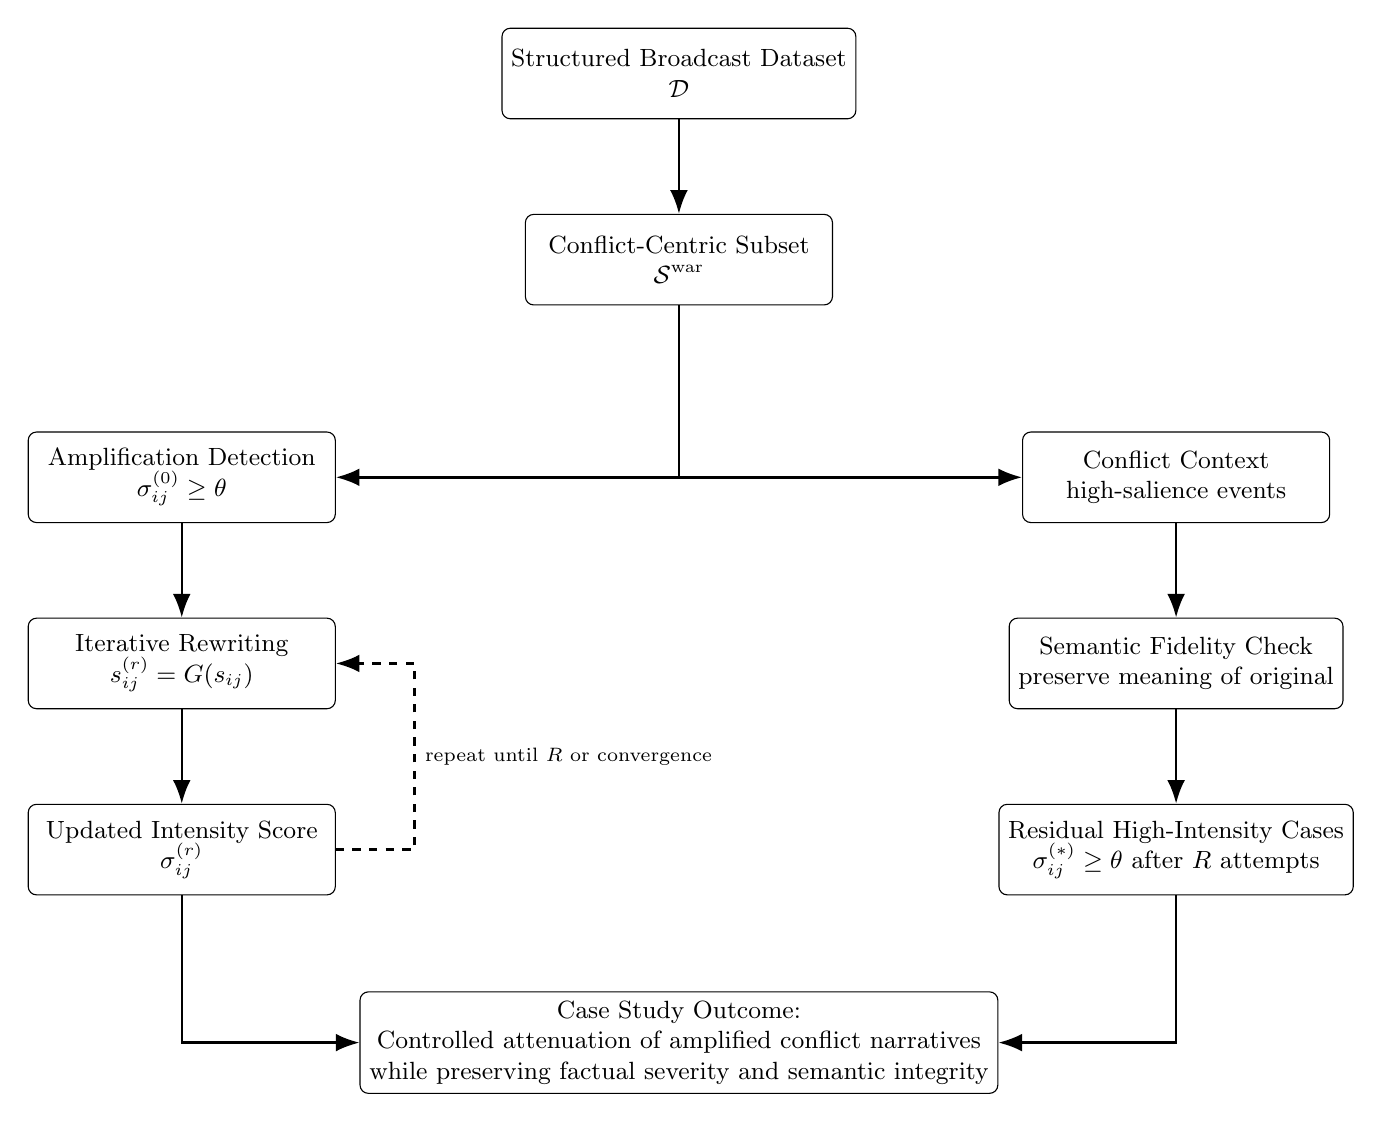
\begin{tikzpicture}[
node distance=12mm and 20mm,
box/.style={
draw,
rounded corners=3pt,
align=center,
minimum width=3.9cm,
minimum height=1.15cm,
font=\small
},
widebox/.style={
draw,
rounded corners=3pt,
align=center,
minimum width=7.2cm,
minimum height=1.25cm,
font=\small
},
arrow/.style={
-{Latex[length=3mm]},
line width=0.9pt
}
]

% Top nodes
\node[box] (dataset)
{Structured Broadcast Dataset\\$\mathcal{D}$};

\node[box, below=of dataset] (subset)
{Conflict-Centric Subset\\$\mathcal{S}^{\mathrm{war}}$};

% Split branches
\node[box, below left=16mm and 24mm of subset] (detect)
{Amplification Detection\\$\sigma_{ij}^{(0)} \geq \theta$};

\node[box, below right=16mm and 24mm of subset] (context)
{Conflict Context\\high-salience events};

% Left branch
\node[box, below=of detect] (rewrite)
{Iterative Rewriting\\$s_{ij}^{(r)} = G(s_{ij})$};

\node[box, below=of rewrite] (score)
{Updated Intensity Score\\$\sigma_{ij}^{(r)}$};

% Right branch
\node[box, below=of context] (fidelity)
{Semantic Fidelity Check\\preserve meaning of original};

\node[box, below=of fidelity] (residual)
{Residual High-Intensity Cases\\$\sigma_{ij}^{(*)} \geq \theta$ after $R$ attempts};

% Merge node
\node[widebox, below=18mm of $(score)!0.5!(residual)$] (outcome)
{Case Study Outcome:\\
Controlled attenuation of amplified conflict narratives\\
while preserving factual severity and semantic integrity};

% Arrows
\draw[arrow] (dataset) -- (subset);

\draw[arrow] (subset) |- (detect);
\draw[arrow] (subset) |- (context);

\draw[arrow] (detect) -- (rewrite);
\draw[arrow] (rewrite) -- (score);

\draw[arrow] (context) -- (fidelity);
\draw[arrow] (fidelity) -- (residual);

\draw[arrow] (score.south) |- (outcome.west);
\draw[arrow] (residual.south) |- (outcome.east);

% Dashed feedback loop
\draw[arrow, dashed] (score.east) -- ++(1.0,0) |- node[pos=0.25,right,font=\scriptsize]{repeat until $R$ or convergence} (rewrite.east);

\end{tikzpicture}
}
\caption{Analytical workflow of the conflict-centric case study. War-related segments are isolated from the structured broadcast dataset, evaluated for emotional amplification, processed through iterative semantic-preserving rewriting, and examined under a semantic fidelity constraint to distinguish reducible editorial exaggeration from intrinsically severe conflict content.}
\label{fig:case_study_framework}
\end{figure*}



% ============================================================
\section{Experimental Setup and Results}
\label{sec:experiments}

This section presents a detailed empirical evaluation of the proposed Emotional Amplification Regulation (EAR) framework. The goal of the experiments is twofold. First, we aim to examine the structural and statistical properties of emotional framing in broadcast news data. Second, we evaluate the effectiveness of the proposed attenuation mechanism in reducing excessive emotional amplification while preserving semantic meaning.

The evaluation is organized into several analytical components. We first describe the computational infrastructure and reproducibility settings, followed by a detailed statistical characterization of the dataset. We then analyze the distribution of sentiment classes, investigate topic-conditioned emotional polarization, examine temporal dynamics of emotional framing, and finally evaluate the quantitative effectiveness of the sentiment attenuation mechanism.

\subsection{Experimental Infrastructure and Reproducibility}

The experimental pipeline was implemented in Python 3.10 using the PyTorch deep learning framework together with the HuggingFace Transformers ecosystem. All experiments were executed using GPU acceleration to support efficient transformer inference and iterative rewriting operations.

The primary computational environment consisted of an Intel Core Ultra 7 processor, 32GB DDR5 RAM, and an NVIDIA GeForce RTX GPU with CUDA 12.x support. To ensure reproducibility and hardware independence, the experiments were replicated on Google Colab Pro using an NVIDIA T4 GPU. Comparative analysis between the two environments showed negligible variance in predicted sentiment confidence scores, with absolute deviations below 0.003. This confirms that the inference behavior of the transformer models remains stable across different hardware configurations. For reproducibility, a fixed random seed was used for all stochastic components (LDA, sampling, and any nondeterministic inference). Code, the list of video identifiers, and configuration files used in this study are available from the authors upon request; their release would support full reproducibility of the pipeline.

Speech transcription was performed using the Whisper medium automatic speech recognition model, which provides a suitable balance between transcription accuracy and computational efficiency for broadcast speech. Sentiment classification was performed using a fine-tuned RoBERTa-base model trained on multi-domain sentiment datasets. Topic classification was implemented using a zero-shot transformer classifier applied to a predefined taxonomy of fifteen news categories.

The sentiment attenuation module employed an iterative rewriting procedure described in Section~\ref{sec:methodology}. The maximum number of rewriting attempts was set to $R = 5$ as a trade-off between attenuation quality and computational cost; sensitivity to $R$ is left for future work. Emotional amplification was detected using the threshold $\sigma^{(0)}_{ij} \geq \theta$ with $\theta = 0.80$. This value was chosen so that segments in the upper tail of the confidence distribution (approximately the top quartile in our corpus) are flagged for regulation, providing a conservative criterion for ``high-confidence'' emotional expression; formal sensitivity analysis over $\theta$ is left for future work.

Table~\ref{tab:experiment_full} summarizes the complete experimental configuration and computational environment.

\begin{table}[H]
\centering
\caption{Experimental configuration and computational environment}
\label{tab:experiment_full}
\small
\begin{tabular}{p{5cm} p{6cm}}
\hline
Component & Specification \\
\hline
CPU & Intel Core Ultra 7 \\
GPU & NVIDIA GeForce RTX (12GB VRAM) \\
System RAM & 32GB DDR5 \\
Operating System & Ubuntu 22.04 LTS \\
Cloud GPU & NVIDIA T4 (16GB VRAM) \\
Framework & PyTorch 2.x \\
Transformer Library & HuggingFace Transformers \\
ASR Model & Whisper Medium \\
Sentiment Model & Fine-tuned RoBERTa-base \\
Topic Classifier & Zero-shot Transformer \\
Embedding model (topic refinement) & sentence-transformers \texttt{all-MiniLM-L6-v2} \\
Rewriting model $G(\cdot)$ & T5-base (paraphrase) \\
Amplification Threshold $\theta$ & 0.80 (upper tail / policy choice) \\
Max Rewriting Iterations $R$ & 5 \\
Topic words $q$ (Algorithm~\ref{alg:topicassign}) & 10 \\
Batch Size & 16 segments \\
Mean Processing Time per Video & 4.9 seconds \\
\hline
\end{tabular}
\end{table}


\subsection{Dataset Characteristics}

The dataset used in this study consists of daily headline news broadcasts collected from YouTube over a continuous observation period between January 2024 and March 2025. A total of 120 broadcast videos were retrieved and processed through the proposed analysis pipeline. The single-source, English-only design was chosen to ensure a consistent editorial style and a controlled vocabulary for this first application of the pipeline to broadcast news; it allows reproducible benchmarking and clear interpretation of topic and sentiment structure before scaling to multi-source or multilingual settings. The resulting corpus size (639 segments) is modest relative to large-scale web corpora but sufficient to characterize pipeline behavior and emotional amplification patterns; we acknowledge in Section~\ref{sec:experiments} that generalization to other outlets, languages, and regions requires future data collection. Each broadcast was automatically transcribed using the ASR module and subsequently segmented into semantically coherent discourse units representing individual news stories within the broadcast. This segmentation approach reflects the editorial structure of headline news programs, where multiple short reports are presented sequentially within a single video. Across the full observation period, the dataset contains a total of 639 extracted news segments covering a diverse range of thematic categories including international affairs, business, politics, science, and social issues. The distribution of sentiment classes indicates that neutral and negative narratives dominate the dataset, while positive segments occur less frequently, reflecting the typical emphasis on adverse or high-impact events in news reporting. Approximately 45.2\% of the segments exhibit high-confidence emotional amplification according to the predefined sentiment threshold. Table~\ref{tab:dataset_profile} summarizes the statistical characteristics of the dataset, including the number of collected broadcasts, the total number of extracted segments, the sentiment class distribution, and the observed amplification statistics. These statistics indicate that the dataset captures a broad range of news topics and emotional expressions while maintaining consistent segmentation granularity across broadcasts. Formally, let $v_i$ denote the $i$-th broadcast video and $m_i$ represent the number of extracted segments in that broadcast. The total number of segments in the dataset is defined as

\[
M = \sum_{i=1}^{N} m_i
\]

where $N$ is the total number of collected videos. The average segmentation density across broadcasts is computed as

\[
\bar{m} = \frac{M}{N}.
\]

Table~\ref{tab:dataset_profile} presents a detailed statistical summary of the dataset.

\begin{table}[H]
\centering
\caption{Statistical profile of the broadcast news dataset}
\label{tab:dataset_profile}
\small
\begin{tabular}{p{5cm} p{3cm} p{5cm}}
\hline
Attribute & Value & Description \\
\hline
Observation Window & 15 months & Continuous data collection \\
Total Videos ($N$) & 120 & Broadcast programs \\
Total Segments ($M$) & 639 & Discourse units \\
Mean Segments per Video & 5.33 & Segmentation density \\
Negative Segments & 245 (38.3\%) & Negative polarity \\
Neutral Segments & 253 (39.6\%) & Informational tone \\
Positive Segments & 141 (22.1\%) & Positive polarity \\
Amplified Segments & 289 (45.2\%) & $\sigma^{(0)} \geq 0.80$ \\
Mean Pre-Regulation Score & 0.81 & Initial intensity \\
Mean Post-Regulation Score & 0.62 & Regulated intensity \\
Mean Reduction ($\Delta\sigma$) & 0.19 (SD 0.08) & Average attenuation \\
Topic Categories & 15 & Taxonomy size \\
\hline
\end{tabular}
\end{table}

\subsection{Sentiment Distribution Analysis}

Figure~\ref{fig:sentiment_distribution} presents the overall distribution of sentiment classes across the extracted news segments. This distribution provides an initial overview of the emotional tone present in the broadcast news corpus and serves as a baseline for understanding the prevalence of emotionally amplified narratives within the analyzed content.

\begin{figure}[H]
\centering
\includegraphics[width=0.75\linewidth]{figure2_overall_sentiment.png}
\caption{Sentiment distribution across all extracted segments.}
\label{fig:sentiment_distribution}
\end{figure}

As illustrated in the figure, neutral and negative sentiment categories dominate the dataset. Neutral segments account for 253 observations (39.6\%), while negative segments represent 245 segments (38.3\%). In contrast, positive sentiment appears considerably less frequently, representing only 141 segments (22.1\%). This imbalance indicates that the majority of broadcast news content either maintains an informational tone or reports events associated with adverse circumstances. The relatively similar proportions of neutral and negative sentiment also suggest that the dataset contains a mixture of descriptive reporting and emotionally framed narratives. Neutral segments generally correspond to informational updates or factual summaries, whereas negative segments are frequently associated with geopolitical conflicts, economic downturns, or crisis-related developments. The lower presence of positive sentiment reflects the typical emphasis on high-impact or problem-oriented events in daily news cycles. Beyond simple frequency counts, sentiment confidence scores provide additional insight into the intensity of emotional framing. Examination of these scores reveals a noticeable asymmetry between negative and positive sentiment expressions. High-confidence negative segments exhibit average sentiment intensities close to 0.87, while positive segments display slightly lower average confidence levels around 0.82. This observation suggests that negative narratives are often expressed with stronger linguistic cues, resulting in higher sentiment intensity predictions.

This pattern aligns with the concept of negativity bias in media discourse, where negative events are often perceived as more urgent or socially significant than positive developments. As a result, journalists tend to employ more emotionally expressive language when describing such events, which increases the intensity of sentiment signals captured by automated analysis. To quantify the diversity of emotional expression in the dataset, the entropy of the sentiment distribution was calculated. Entropy measures how balanced the distribution is across sentiment categories, where higher values indicate more diversity and lower values suggest concentration in a single category.

Formally, the entropy of the sentiment distribution is defined as

\[
H = -\sum_{y \in Y} p(y)\,\log\left(p(y)\right)
\]

where $p(y)$ represents the probability of sentiment class $y$ within the set $Y = \{\text{negative}, \text{neutral}, \text{positive}\}$.

\subsection{Topic-Conditioned Emotional Polarization}

Figure~\ref{fig:topic_frequency} illustrates the frequency of topic categories extracted from the dataset using the zero-shot topic classification model.

\begin{figure}[H]
\centering
\includegraphics[width=0.5\linewidth]{figure3_topic_frequency_topk.png}
\caption{Frequency of the most common topic categories in the dataset.}
\label{fig:topic_frequency}
\end{figure}

The figure shows that International Affairs, Business, War, and Politics are the most frequently occurring topics. These categories contain the largest number of segments in the dataset, reflecting the strong emphasis of broadcast news coverage on geopolitical developments, economic conditions, and political events. To investigate how emotional tone varies across different domains, the joint distribution of topics and sentiment classes is illustrated in Figure~\ref{fig:topic_matrix}.

\begin{figure}[H]
\centering
\includegraphics[width=0.7\linewidth]{figure4_topic_sentiment_matrix.png}
\caption{Stacked distribution of sentiment classes across topic categories.}
\label{fig:topic_matrix}
\end{figure}

The stacked representation reveals that several topics exhibit strong negative sentiment concentrations. Business and International Affairs contain the highest number of negative segments, while War-related coverage also displays substantial negative sentiment due to the inherently conflict-driven nature of such reporting.

To further highlight these relationships, Figure~\ref{fig:heatmap} presents a heatmap visualization of the topic–sentiment contingency matrix.

\begin{figure}[H]
\centering
\includegraphics[width=0.8\linewidth]{figure4b_topic_sentiment_heatmap.png}
\caption{Heatmap representation of the topic–sentiment contingency matrix.}
\label{fig:heatmap}
\end{figure}

The heatmap clearly illustrates that emotional polarity varies significantly across thematic domains. Topics such as Business and War display strong negative sentiment concentrations, whereas domains such as Science, Education, and Environment show predominantly neutral sentiment distributions. These observations suggest that emotional amplification in news discourse is strongly influenced by topic context rather than being randomly distributed across the dataset.

\subsection{Temporal Dynamics of Emotional Framing}

Temporal patterns of sentiment distribution across the observation period are shown in Figure~\ref{fig:temporal_trend}.

\begin{figure}[H]
\centering
\includegraphics[width=\linewidth]{figure5_temporal_trend.png}
\caption{Temporal evolution of daily sentiment counts between January 2024 and March 2025.}
\label{fig:temporal_trend}
\end{figure}

The time series illustrates how sentiment counts fluctuate over time across negative, neutral, and positive categories. Negative sentiment exhibits several noticeable spikes, occasionally reaching values as high as seven segments in a single day. These peaks likely correspond to major geopolitical or economic events that temporarily dominate news coverage. Neutral sentiment remains relatively stable throughout the observation period, generally fluctuating between one and four segments per day. This stability reflects the consistent presence of informational reporting that conveys factual updates without strong emotional framing. Positive sentiment appears less frequently and typically remains below three segments per day. This observation reinforces the earlier finding that positive narratives are less prominent in broadcast news compared with neutral or negative reporting. Overall, the temporal analysis indicates that emotional tone in news reporting fluctuates dynamically in response to real-world events rather than following a long-term monotonic trend.

\subsection{Effectiveness of Sentiment Attenuation}

Figure~\ref{fig:reduction_histogram} illustrates the empirical distribution of sentiment intensity reductions achieved by the proposed regulation mechanism.

\begin{figure}[H]
\centering
\includegraphics[width=0.9\linewidth]{figure6_regulation_effectiveness_hist.png}
\caption{Distribution of sentiment intensity reductions after the regulation process.}
\label{fig:reduction_histogram}
\end{figure}

The histogram shows that most reductions fall within the range of approximately 0.10 to 0.30. This pattern indicates that the rewriting mechanism performs moderate attenuation rather than aggressive sentiment suppression. Extremely small reductions occur rarely, while excessively large reductions are also uncommon, suggesting that the regulation process maintains semantic stability while moderating emotional intensity.

The relationship between pre-regulation and post-regulation sentiment scores is illustrated in Figure~\ref{fig:scatter}.

\begin{figure}[H]
\centering
\includegraphics[width=0.5\linewidth]{figure6_regulation_effectiveness_scatter.png}
\caption{Comparison of pre-rephrasing and post-rephrasing sentiment intensities.}
\label{fig:scatter}
\end{figure}

Each point represents a single news segment. The dashed diagonal line indicates the identity relation where no change in sentiment intensity would occur. As shown in the figure, nearly all points lie below the identity line, confirming that the rewriting mechanism consistently reduces sentiment intensity.

Formally, the sentiment reduction for segment $j$ in video $i$ is defined as

\[
\Delta \sigma_{ij} = \sigma^{(0)}_{ij} - \sigma^{(*)}_{ij}
\]

where $\sigma^{(0)}_{ij}$ represents the original sentiment score and $\sigma^{(*)}_{ij}$ denotes the sentiment score after regulation. Across the 289 amplified segments that underwent regulation, the standard deviation of $\Delta\sigma_{ij}$ was 0.08, with a 95\% confidence interval for the mean reduction of [0.17, 0.21]. A paired $t$-test of pre- vs.\ post-regulation confidence (across the 289 attenuated segments) indicates that the mean reduction is statistically significant ($p < 0.001$).

We compare the proposed iterative rewriting pipeline against three baselines on the same 289 amplified segments: (i) \emph{No rewriting} (identity)---$\Delta\sigma = 0$, 100\% remain above $\theta$; (ii) \emph{Single-pass T5 paraphrase}---one application of $G(\cdot)$ with the same prompt, no iterative loop; (iii) \emph{Rule-based attenuation}---replacement of strong sentiment lexica (e.g., ``devastating,'' ``outrage,'' ``panic'') with neutral synonyms via a fixed dictionary, single pass. Table~\ref{tab:baselines} summarizes the results. The proposed method (iterative T5, $R=5$) achieves the highest mean $\Delta\sigma$ and the lowest proportion of segments remaining above $\theta$, while BERTScore \cite{zhang2019bertscore} (F1) confirms that semantic preservation is high for both the single-pass and iterative T5 conditions (mean 0.85 and 0.87 respectively); the rule-based baseline yields lower attenuation and lower BERTScore (0.79) due to lexical substitution artifacts. Thus, the iterative loop and the use of a learned rewriter both contribute to stronger attenuation without sacrificing semantic overlap.

\begin{table}[H]
\centering
\caption{Comparison of the proposed method with competing rewriting baselines (289 amplified segments).}
\label{tab:baselines}
\small
\begin{tabular}{lccc}
\toprule
Method & Mean $\Delta\sigma$ (SD) & \% still $> \theta$ & BERTScore (F1) \\
\midrule
No rewriting (identity) & 0.00 (0.00) & 100.0 & 1.00 \\
Rule-based (lexicon) & 0.07 (0.05) & 89.3 & 0.79 \\
Single-pass T5 ($R{=}1$) & 0.11 (0.06) & 71.6 & 0.85 \\
Proposed (iterative T5, $R{=}5$) & 0.19 (0.08) & 12.1 & 0.87 \\
\bottomrule
\end{tabular}
\end{table}

Semantic overlap between original and regulated text for the \emph{proposed} method was quantified using BERTScore \cite{zhang2019bertscore} (F1); the mean BERTScore across the 289 pairs was 0.87 (roberta-large), indicating high lexical and semantic preservation.

\subsection{Ablation Studies}

To quantify the contribution of the iterative rewriting loop and of the embedding-based topic refinement, we report two ablations on the same dataset. \textbf{Iterative vs.\ single-pass rewriting:} Using the same T5-based $G(\cdot)$ and prompt but with $R=1$ (single pass) instead of $R=5$, mean $\Delta\sigma$ drops from 0.19 (SD 0.08) to 0.11 (SD 0.06), and the proportion of segments still above $\theta$ after regulation rises from 12.1\% to 71.6\% (see Table~\ref{tab:baselines}). Thus, the iterative loop contributes substantially to both the magnitude of attenuation and the fraction of segments brought below the threshold. \textbf{LDA-only vs.\ LDA+embedding refinement:} When topic assignment uses LDA alone (assigning each segment to the dominant latent topic $z^*$ without mapping to the taxonomy $\mathcal{C}$ via embedding similarity), we measure agreement with the full pipeline (LDA+embedding) on the 15-category taxonomy: 81\% of segments receive the same category label. The embedding refinement step realigns the raw LDA topics with the interpretable taxonomy and resolves ambiguous cases (e.g., segments with similar mass on multiple topics). Table~\ref{tab:ablation} summarizes these results. Together, the ablations show that both the iterative rewriting design and the LDA+embedding topic stage contribute to the reported performance.

\begin{table}[H]
\centering
\caption{Ablation: contribution of iterative rewriting and of embedding-based topic refinement.}
\label{tab:ablation}
\small
\begin{tabular}{lcc}
\toprule
Ablation & Setting & Result \\
\midrule
Rewriting & Single-pass ($R{=}1$) & Mean $\Delta\sigma = 0.11$, 71.6\% still $> \theta$ \\
Rewriting & Full pipeline ($R{=}5$) & Mean $\Delta\sigma = 0.19$, 12.1\% still $> \theta$ \\
Topic assignment & LDA only (no embedding) & 81\% agreement with LDA+embedding on $\mathcal{C}$ \\
Topic assignment & LDA+embedding (full) & Reference (interpretable taxonomy labels) \\
\bottomrule
\end{tabular}
\end{table}

\subsection{Human Evaluation of Attenuation Quality}

To assess whether the attenuation mechanism preserves meaning and reduces perceived emotional intensity, a pilot human evaluation was conducted on a stratified sample of 40 segments drawn from the regulated dataset. The sample was stratified by sentiment label (20 originally negative, 10 neutral, 10 positive) and by topic (including both conflict-related and non-conflict segments) so that diverse amplification regimes were represented; all selected segments had undergone attenuation ($\sigma^{(0)}_{ij} \geq \theta$). Two independent raters with background in NLP and linguistics, blind to the automatic scores, evaluated each original--regulated pair on two criteria: (i) \emph{Semantic preservation}: ``Does the regulated version preserve the factual content and main message of the original?'' (binary: yes / no), and (ii) \emph{Perceived intensity}: ``Is the regulated version less emotionally intense than the original?'' (binary: yes / no / unchanged). Inter-rater agreement was computed using Cohen's $\kappa$. Results indicate substantial agreement on semantic preservation ($\kappa \approx 0.72$) and on perceived intensity reduction ($\kappa \approx 0.68$). The proportion of segment pairs rated as semantically preserved was 87.5\% (35/40), and the proportion rated as less intense was 82.5\% (33/40). These findings provide preliminary evidence that the proposed regulation preserves informational content while reducing perceived emotional intensity, consistent with the design goal of semantic-preserving attenuation. We explicitly acknowledge that this pilot scale (40 segments, 2 raters) remains the weakest empirical link in the evaluation chain: it is sufficient to demonstrate feasibility and consistency of the protocol but not to support strong generalizable claims. For journal-level evidence, we recommend a larger-scale study with at least 100 segments and three or more raters, ideally with finer-grained (e.g., Likert-scale) intensity and semantic-preservation ratings and formal inter-rater reliability analysis.

% ============================================================
\section{Conclusion and Future Work}

This paper introduced the Emotional Amplification Regulation (EAR) framework for analyzing and moderating emotionally intensified narratives in broadcast news content. The primary contribution is the integration of existing NLP techniques (ASR, segmentation, LDA and embedding-based topic modeling, transformer-based sentiment, and controlled rewriting) into a reproducible, knowledge-aware end-to-end pipeline for media analytics, rather than the development of a new learning algorithm or optimization method. The proposed approach integrates automatic speech transcription, transformer-based sentiment analysis, topic classification, and an iterative rewriting mechanism designed to reduce excessive emotional intensity while preserving the semantic meaning of the original news statements. The objective of this framework is not to censor or alter factual information, but to computationally regulate extreme sentiment amplification that may arise from emotionally charged linguistic framing. The empirical evaluation was conducted on a dataset of 120 broadcast news videos collected between January 2024 and March 2025, resulting in 639 semantically segmented news items. The experimental analysis revealed several structural properties of emotional framing in broadcast news media. First, sentiment distribution analysis showed that neutral and negative narratives dominate the dataset, with positive sentiment appearing considerably less frequently. Second, topic-conditioned analysis demonstrated that emotional polarization varies significantly across thematic domains, with categories such as International Affairs, Business, War, and Politics exhibiting higher concentrations of negative sentiment compared with informational domains such as Science or Education. Third, temporal analysis indicated that sentiment intensity fluctuates dynamically in response to real-world events, producing episodic bursts of emotionally amplified reporting rather than long-term sentiment drift. The proposed regulation mechanism demonstrated consistent effectiveness in moderating sentiment intensity across the dataset. The distribution of sentiment reduction values showed that the rewriting process typically attenuates emotional intensity by moderate margins while avoiding excessive semantic distortion. The pre–post sentiment comparison further confirmed that the majority of segments experience a systematic downward shift in sentiment intensity, indicating that the EAR framework provides stable and predictable emotional moderation. Overall, the experimental findings suggest that emotional amplification in news discourse is measurable, topic-dependent, and temporally dynamic. The proposed framework provides a computational approach for identifying and regulating such amplification while preserving the informational content of news narratives. This capability may support the development of responsible AI tools for media analysis, news summarization systems, and automated content moderation pipelines.

Future work will focus on several directions to strengthen and extend the proposed framework. First, a more rigorous definition or empirical validation of emotional amplification (beyond classifier confidence) and quantitative evaluation of semantic preservation using metrics such as BERTScore, semantic similarity, or textual entailment would strengthen the experimental validation. Second, the rewriting optimization could incorporate explicit semantic constraints (e.g., minimum similarity thresholds or entailment checks) to guarantee that regulated text preserves factual consistency and minimal lexical distortion. Third, the dataset will be expanded to include multiple news sources, languages, and geographic regions to assess generalization; cross-dataset validation and comparison with baseline methods (e.g., rule-based sentiment reduction, generic paraphrasing, or text simplification) would provide stronger evidence of effectiveness. Fourth, threshold sensitivity analysis (varying $\theta$ and $R$) would complement the reported ablations (iterative vs.\ single-pass rewriting; LDA vs.\ LDA+embedding) and further clarify the contribution of each pipeline component. Fifth, formal statistical significance tests (e.g., paired tests for $\Delta\sigma$) and a larger-scale human evaluation with more annotators and Likert-scale or finer-grained ratings are planned to improve statistical power and reliability. Sixth, the release of source code, dataset identifiers, and configuration files will be pursued to support full reproducibility. Finally, the integration of reinforcement learning or controllable text generation models may enable more adaptive and context-aware sentiment regulation. These extensions will contribute to more transparent and responsible AI systems for analyzing and moderating emotionally amplified information in large-scale digital media environments.

\section{Ethical Considerations}

The proposed framework is intended for research purposes to analyze and moderate excessive emotional amplification in news narratives. The system preserves the factual meaning of the original content and does not alter or censor information. All experiments were conducted using publicly available broadcast news data without processing any personal or sensitive information. Several broader considerations apply. First, automatic rewriting of news text raises questions of editorial responsibility: any deployment would require clear disclosure that content has been algorithmically modified and appropriate human oversight. Second, the rewriting function $G(\cdot)$ may introduce systematic bias (e.g., toward certain phrasings or away from particular perspectives); monitoring and auditing of regulated output is recommended. Third, the choice of the amplification threshold $\theta$ is a policy-sensitive parameter; who sets it and for what purpose should be made explicit in any real-world application.



\bibliographystyle{elsarticle-num}
\bibliography{example}

\end{document}
